% Section content template for individual Educative lessons
% This file contains the actual content for a specific section
% Generated from Educative API section content

% Section: Design of Yelp
% Section ID: 5027439944400896
% Section Slug: design-of-yelp
% Generated: 2025-12-07T23:22:20.857705

We identified the requirements and calculated the estimations for our Yelp system in the previous lesson. In this lesson, we discuss the API design, go through the storage schema, and then dive into the details of the system's building blocks and additional components.

\subsection{API design}\label{05mmmSTJ18Mes17g9mklG}
\\
Let's discuss the API design for Yelp.

\subsubsection{Search}\label{SOk21pVYaTlvzplH6qWmK}
\\
We need to implement the \texttt{search} function. The API call for searching based on categories like ``cafes'' will be:

\begin{lstlisting}[language=JavaScript]
search(category, user_location, radius)
\end{lstlisting}

\begin{table}[htbp]
\centering
\small
\adjustbox{max width=\textwidth}{
\begin{tabular}{|p{0.303\textwidth}|p{0.647\textwidth}|}
\hline
\textbf{Parameter} & \textbf{Description} \\
\hline
\hline
\texttt{category} & This is the type of search the user makes---for example, a search for restaurants, cinemas, cafes, and so on. \\
\hline
\texttt{user\_location} & This contains the location of the user who's searching with Yelp. \\
\hline
\texttt{radius} & This is the specified radius where the user is trying to find the required category. \\
\hline
\end{tabular}
}
\end{table}

This process returns a JSON object that contains a list of all the possible items in the specified category that also fall within the specified radius. Each entry has a place name, address, category, rating, and thumbnail.
\\
The API call for searching based on the name of a place like ``Burger Hut'' will be:

\begin{lstlisting}[language=JavaScript]
search(name_of_place, user_location, radius)
\end{lstlisting}

\begin{table}[htbp]
\centering
\small
\adjustbox{max width=\textwidth}{
\begin{tabular}{|p{0.303\textwidth}|p{0.647\textwidth}|}
\hline
\textbf{Parameter} & \textbf{Description} \\
\hline
\hline
\texttt{name\_of\_place} & This contains the name of the place that the user wants to search for. \\
\hline
\end{tabular}
}
\end{table}

This process returns a JSON object that contains information of the specified place.

\subsubsection{Add a place}\label{I69uuTzlyrN_rd36-yCz1}
\\
The API call for adding a place is below:

\begin{lstlisting}[language=JavaScript]
add_place(name_of_place, description_of_place, category, latitude, longitude, photo}
\end{lstlisting}

\begin{table}[htbp]
\centering
\small
\adjustbox{max width=\textwidth}{
\begin{tabular}{|p{0.303\textwidth}|p{0.647\textwidth}|}
\hline
\textbf{Parameter} & \textbf{Description} \\
\hline
\hline
\texttt{name\_of\_place} & This contains the name of the place, for example, "Burger Hut". \\
\hline
\texttt{description\_of\_place} & This contains a description of the place. For example, "Burger Hut sells the yummiest burgers". \\
\hline
\texttt{category} & This specifies the category of the place---for example, "cafe". \\
\hline
\texttt{latitude} & This tells us the latitude of the place. \\
\hline
\texttt{longitude} & This tells us the longitude of the place. \\
\hline
\texttt{photo} & This contains photos of the place. There can be a single or multiple photos. \\
\hline
\end{tabular}
}
\end{table}

This process returns a response saying that a place has been added, or an appropriate error if it fails to add a place.

\subsubsection{Add a review}\label{G9ihCBTrmXrFysp16_ygh}
\\
The API call for adding a review is below:

\begin{lstlisting}[language=JavaScript]
add_review(place_ID, user_ID, review_description, rating)
\end{lstlisting}

\begin{table}[htbp]
\centering
\small
\adjustbox{max width=\textwidth}{
\begin{tabular}{|p{0.303\textwidth}|p{0.647\textwidth}|}
\hline
\textbf{Parameter} & \textbf{Description} \\
\hline
\hline
\texttt{place\_ID} & This contains the ID of the place whose review is added. \\
\hline
\texttt{user\_ID} & This contains the ID of the user who adds the review. \\
\hline
\texttt{review\_description} & This contains the review of the place---for example, "the food and ambiance were superb". \\
\hline
\texttt{rating} & This contains the rating of the place---for example, 4 out of 5. \\
\hline
\end{tabular}
}
\end{table}

This process returns a response that a review has been added, or an appropriate error if it fails to add a review.

\subsection{Storage schema}\label{umw_dT_-eJdkCm7Fuq7U1}
\\
Let's define the storage schema for our system. A few of the tables we might need are ``Place,'' ``Photos,'' ``Reviews,'' and ``Users.''
\\
Let's define the columns of the ``Place'' table:

\begin{itemize}
\item
\protect\phantomsection\label{7gimEx9hB33VI8vEvIcMv}
\textbf{Place\_ID}: We use the sequencer to generate an 8 Bytes (64 bits) unique ID for a place.
\end{itemize}
\begin{quote}
\textbf{Note:}~We generate IDs using the unique ID generator.
\end{quote}
\begin{itemize}
\item
\protect\phantomsection\label{Kz0Dhe-o2wSe1aCefw86A}
\textbf{Name\_of\_Place}: This is a string that contains the name of the place. We use 256 Bytes for it.
\item
\protect\phantomsection\label{MYVVj0QtL69h3ZAH_58NR}
\textbf{Description\_of\_Place}: This holds a description of the place. We use 1,000 Bytes for it.
\item
\protect\phantomsection\label{IaBYZTbgKXcsByRgd5dKG}
\textbf{Category}: This specifies the type of place like restaurants, cinemas, bookshops, and so on (8 Bytes).
\item
\protect\phantomsection\label{vPj8RCrgR3Io6ER72ck3C}
\textbf{Latitude}: This stores the latitude of the location (8 Bytes).
\item
\protect\phantomsection\label{g8cuT1I_-EkX1CkOir3Sn}
\textbf{Longitude}: This stores the longitude of the location (8 Bytes).
\item
\protect\phantomsection\label{UstnpBzayge0odONQehPk}
\textbf{Rating}: This stores the rating of the place. It shows how many stars a place gets out of five. The rating is calculated based on the reviews it gets from the users.
\end{itemize}
\\
The columns mentioned above are the most important ones in the table. We can add more columns like ``menu,'' ``address,'' ``opening and closing hours,'' and so on. Therefore, keeping in mind the essential columns, the size of one row of our table will be:

\begin{lstlisting}[language=JavaScript]
Size = 8 + 256 + 1000 + 8 + 8 + 8 + 1 = 1289 bytes
\end{lstlisting}

Now let's define the ``Photos'' table:

\begin{itemize}
\item
\protect\phantomsection\label{5-WTF3QtS-ISgFm47mO5Y}
\textbf{Photo\_ID}: We use the sequencer to generate a unique ID for a photo (8 Bytes or 64 bits).
\item
\protect\phantomsection\label{KQnaoXkAHrgQximObjUMt}
\textbf{Place\_ID}: We use the foreign key (8 Bytes) from the ``Place'' table to identify which photo belongs to which place.
\item
\protect\phantomsection\label{bCTNRCcSEq_4yxwvqAQ79}
\textbf{Photo\_path}: We store the photos in blob storage and save the photo's path (256 Bytes) in this column.
\end{itemize}

\begin{lstlisting}[language=JavaScript]
Size = 8 + 8 + 8 + 256 = 280 bytes
\end{lstlisting}

We need another table called ``Reviews'' to store the reviews, ratings, and photos of a place.

\begin{itemize}
\item
\protect\phantomsection\label{NkA4pfgIDzd47o1DAUMV7}
\textbf{Review\_ID}: We use the sequencer to generate a unique ID of 8 Bytes (64 bits) for a review.
\item
\protect\phantomsection\label{Ysvt-RlT5P2zIzdn1NMBr}
\textbf{Place\_ID}: The foreign key (8 Bytes) from the ``Place'' table to determine which place the rating belongs to.
\item
\protect\phantomsection\label{hGmiUH7Bf3Etq_PQgEIEQ}
\textbf{User\_ID}: The foreign key (8 Bytes) from the ``Users'' table to identify which review belongs to which user.
\item
\protect\phantomsection\label{0xe3evyDJSrduK064PQSj}
\textbf{Review\_description}: This holds a description of the review. We use 512 Bytes for it.
\item
\protect\phantomsection\label{6y_voqgVKgVXaKUJdysF2}
\textbf{Rating}: This stores how many stars a place gets out of five (1 Byte).
\end{itemize}

\begin{lstlisting}[language=JavaScript]
Size = 8 + 8 + 8 + 512 + 1 = 537 bytes
\end{lstlisting}

We use the ``Users'' table to store user information.

\begin{itemize}
\item
\protect\phantomsection\label{tPfeRttSayXFLIamV-nVl}
\textbf{User\_ID}: We use the sequencer to generate a unique ID for a user (8 Bytes).
\item
\protect\phantomsection\label{_Jh6tRLOjmcUqOBHE7Lgt}
\textbf{User\_name}: This is a string that contains the user's name. We use 256 Bytes for it.
\end{itemize}

\begin{lstlisting}[language=JavaScript]
Size = 8 + 256 = 264 bytes
\end{lstlisting}

\begin{quote}
\textbf{Note:} The \texttt{INT} in the following schema contains an 8-Byte ID that we generate using the unique ID generator.
\end{quote}

\begin{figure}[htbp]
 \centering
 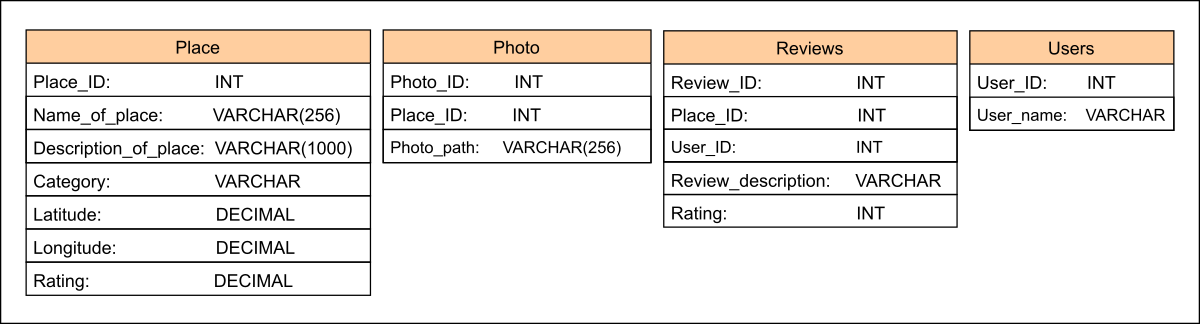
\includegraphics[width=0.5\textwidth]{Images/chapter_29/section_5027439944400896/6713891328753664.png}
 \caption{Storage schema}
\end{figure}

\subsection{Design}\label{MEke93DNw326ZMngq-VbB}
\\
Now we'll discuss the individual building blocks and components used in the design of Yelp and how they work together to complete various functional requirements.

\subsubsection{Components}\label{lZArUWs3MX8n8N0nKU3lc}
\\
These are the components of our system:

\begin{itemize}
\item
\protect\phantomsection\label{snMvXjbUSB6ZBU-uaJk-Y}
\textbf{Segments producer}: This component is responsible for communicating with the third-party world map data services (for example, Google Maps). It takes up that data and divides the world into smaller regions called segments. The segment producer helps us narrow down the number of places to be searched.
\item
\protect\phantomsection\label{sTkX98yQd3t6N3KG9Oxqd}
\textbf{QuadTree servers}: These are a set of servers that have trees that contain the places in the segments. A QuadTree server finds a list of places based on the given radius and the user's provided location and returns that list to the user. This component mainly aids the search functionality.
\item
\protect\phantomsection\label{okpBfPHTQVpVjtZLMs5je}
\textbf{Aggregators}: The QuadTrees accumulate all the places and send them to the aggregators. Then, the aggregators aggregate the results and return the search result to the user.
\item
\protect\phantomsection\label{b7R7b6Pbdo26CS_S7yDwZ}
\textbf{Read servers}: We use a set of read servers that we use to handle all the read requests. Since we have more read requests, it's efficient to separate these requests from the write requests. Each read server directs the search requests to the QuadTrees' servers and returns the results to the user.
\item
\protect\phantomsection\label{-7QVDA0-4PJFmaWwNdZ8R}
\textbf{Write server}: We use a set of write servers to handle all the write requests. Each write server handles the write requests of the user and updates the storage accordingly. Examples for write requests include adding a place, writing a comment, rating a place, and so on.
\item
\protect\phantomsection\label{2MVItd7KK_v9TJOmj98mi}
\textbf{Storage}: We'll use two types of storage to fulfill our diverse needs.

\begin{itemize}
\item
\textbf{SQL database}: Our system will have different tables like ``Users,'' ``Place,'' ``Reviews,'' ``Photos,'' and others as described below. The data in these tables is inherently relational and structured. We need to perform queries like places a user visited, reviews they added, or view all the reviews of a specific place. It's easy to perform such queries in a SQL-based database. We also want all users to have a consistent view of the data, and SQL-based databases are better suited for such use cases. We'll use reliable and scalable databases, as is discussed in the \href{https://www.educative.io/courses/grokking-the-system-design-interview/introduction-to-databases}{Database} building block.
\item
\textbf{Key-value stores}: We'll need to fetch the places in a segment efficiently. For that, we store the list of places against a segment ID in a key-value store to minimize searching time. We also save the QuadTree information in the key-value store, by storing the QuadTree data against a unique ID.
\end{itemize}
\item
\protect\phantomsection\label{bPRGntBziGy7xHP1ZblBE}
\textbf{Load balancer}: A load balancer distributes users' incoming requests to all the servers uniformly.
\end{itemize}

\begin{figure}[htbp]
 \centering
 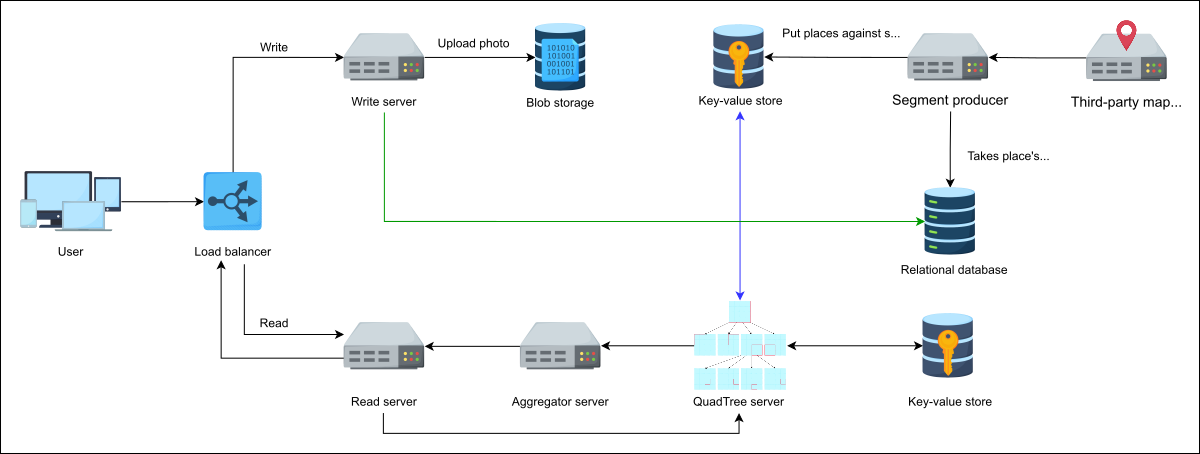
\includegraphics[width=0.5\textwidth]{Images/chapter_29/section_5027439944400896/5351631685550080.png}
 \caption{The detail design of Yelp}
\end{figure}

\subsubsection{Workflow}\label{-ExyyWXGsPZ46cCxnl_bY}
\\
The user puts in a search request. We find all the relevant places in the given radius, while considering the user's location (latitude, longitude).
\\
We explain the detailed workflow of our system in terms of the required functionalities below:

\begin{itemize}
\item
\protect\phantomsection\label{zGrqtD52QJbiJqG-W8CmB}
\textbf{Searching a place}: The load balancers route read requests to the read servers upon receiving them. The read servers direct them to the QuadTree servers to find all the places that fall within the given radius. The QuadTree servers then send the results to the aggregators to refine them and send them to the user.
\item
\protect\phantomsection\label{pYHGnxk1fhJ_Na2IQ5NJK}
\textbf{Adding a place or feedback}: The load balancers route the write requests to the write servers upon receiving them. Depending on the provided content, meaning the place information or review, the write servers add an entry in the relational database and put all the related images in the blob storage.
\item
\protect\phantomsection\label{t8hsQzp0E9S3E4KT6uoOM}
\textbf{Making segments}: The segment's producer splits the world map taken from the third-party map service into smaller segments. The places inside each segment are stored in a key-value store. Even though this is a one-time job, this process is repeated periodically for newer segments and places. Since the probability of new places being added is low, we update our segments every month.
\end{itemize}
\\
We've discussed the design of Yelp, its API design, and the relevant storage schema. In the next lesson, we'll talk about the design considerations.

% End of section content